\documentclass{article}

\usepackage{iclr2026_conference,times}
\usepackage{amsmath}
\usepackage{amssymb}
\usepackage{amsthm}
\usepackage{booktabs}
\usepackage{graphicx}
\usepackage{url}

\newtheorem{proposition}{Proposition}
\newtheorem{definition}{Definition}

\title{Mechanism-First Repair Coordinates for Sim-to-Real Adaptation}

\author{Anonymous Authors}

\begin{document}

\maketitle

\begin{center}
{\small Submission-hardening version: v2 (2026-06-12).}
\end{center}

\begin{abstract}
Most sim-to-real pipelines adapt policies, simulator parameters, domain statistics, or latent context variables. This paper studies a smaller but consequential alternative: adapt the mechanism of failure that determines the repair. We formalize a repair-aliasing boundary in which two target domains share the same passive deployment statistic but require incompatible repairs, making any statistic-only adapter fail on at least one domain. We then introduce mechanism-first repair coordinates: short diagnostic interventions produce residual signatures that classify the target into a repair-equivalence class before controller repair is selected. A runnable contact-control simulator instantiates actuator gain loss, actuation delay, high-command slip, and contact compliance under nuisance-heavy shifts. In this simulator, mechanism-first probing matches the mechanism oracle and reduces mean final error from $0.0076$ for a coarse passive-statistic oracle to $0.0017$, while no adaptation and nuisance nearest-neighbor baselines are substantially worse. The v2 probe-noise stress narrows the claim: mechanism classification is perfect only with clean hand-designed probes; at probe noise $\sigma=0.04$ accuracy falls to 0.830 and mean final error rises to 0.0294, and at $\sigma=0.12$ accuracy falls to 0.503 with mean final error 0.1098. The result is not hardware evidence and is not a universal argument against domain randomization or system identification. It is a constructive boundary case showing that, when repair-critical mechanisms are aliased by domain summaries, the adaptation coordinate itself matters.
\end{abstract}

\section{Introduction}

Sim-to-real transfer is often framed as a coverage or alignment problem: randomize enough simulator factors, estimate the target dynamics, learn a domain-invariant representation, or adapt a residual policy until deployment behavior improves \citep{tobin2017domain,peng2018dynamics,tan2018agile,yu2017uposi,chebotar2019closing,muratore2022robot}. These coordinates are useful, but they can be mismatched to a deployment decision. A robot does not always need the full target domain distribution. It often needs to know which repair to apply: compensate actuator gain, predict through delay, avoid slip-inducing commands, preload a compliant contact, or stop because the failure is out of library.

This paper asks what changes if the deploy-time object of adaptation is the failure mechanism that determines the repair. The answer is not ``more data'' or a larger policy. The central mechanism is a repair-equivalence coordinate: target domains are grouped by the intervention that makes the controller work, even when their nuisance variables or exact physical parameters differ.

The contribution is intentionally narrow.
\begin{itemize}
    \item We define repair aliasing and prove a small boundary result: if two domains have the same statistic but different margin-separated optimal repairs, any adapter that observes only that statistic must incur regret on at least one.
    \item We propose mechanism-first repair selection, where short diagnostic probes expose residual signatures for repair-equivalence classes.
    \item We provide a runnable contact-control simulator with four embodied failure mechanisms and nuisance-heavy shifts. The experiment demonstrates the coordinate mismatch in a controlled setting.
    \item We provide a 1500-paper landscape matrix, a 100-paper hostile prior-work set, and an explicit claim audit to keep the novelty boundary honest.
\end{itemize}

We do not claim real-robot superiority, broad replacement of domain randomization, or a solved open-world failure taxonomy. The evidence supports a more modest thesis: some sim-to-real failures are not primarily failures of optimization over the chosen statistic; they are failures caused by choosing the wrong adaptation coordinate.

\section{Problem Setting}

Let $d \in \mathcal{D}$ denote a target deployment domain. A robot observes limited deployment information and must choose a repair $r \in \mathcal{R}$ before executing a controller. The loss $L(d,r)$ measures task error, safety cost, or negative reward after applying repair $r$ in domain $d$.

\begin{definition}[Repair-equivalence]
Two domains $d_i,d_j$ are repair-equivalent under loss $L$ and repair set $\mathcal{R}$ if
\[
\arg\min_{r\in \mathcal{R}} L(d_i,r) = \arg\min_{r\in \mathcal{R}} L(d_j,r).
\]
A mechanism-first adapter estimates this equivalence class, not necessarily the full domain or simulator parameter vector.
\end{definition}

Many sim-to-real methods implicitly use a statistic $\sigma(d)$: visual appearance features, nominal rollout outcomes, estimated dynamics parameters, randomized-domain embeddings, or learned latent context. These statistics can be repair-relevant, but they need not be. The failure mode studied here is that $\sigma$ aliases domains that require different repairs.

\begin{proposition}[Repair aliasing for statistic-only adapters]
Assume there exist two domains $d_a,d_b$ and two distinct repairs $r_a,r_b$ such that $\sigma(d_a)=\sigma(d_b)$, $r_a$ is the unique optimal repair for $d_a$, $r_b$ is the unique optimal repair for $d_b$, and every non-optimal repair has regret at least $\Delta>0$ in its domain. Then any deterministic adapter $g(\sigma(d))$ incurs regret at least $\Delta$ on either $d_a$ or $d_b$. Any randomized adapter that conditions only on $\sigma(d)$ incurs expected regret at least $\Delta/2$ under the uniform distribution over $\{d_a,d_b\}$.
\end{proposition}

\begin{proof}
Since $\sigma(d_a)=\sigma(d_b)$, a deterministic statistic-only adapter must return the same repair for both domains. If it returns $r_a$, it is non-optimal on $d_b$ and has regret at least $\Delta$; if it returns $r_b$, it is non-optimal on $d_a$; any other repair is non-optimal on both. For a randomized adapter, let $p_a$ and $p_b$ be the probabilities assigned to $r_a$ and $r_b$ after observing the shared statistic. The expected regret is at least
\[
\frac{\Delta}{2}(1-p_a) + \frac{\Delta}{2}(1-p_b)
= \Delta\left(1-\frac{p_a+p_b}{2}\right).
\]
Because $r_a\neq r_b$, $p_a+p_b\leq 1$, so the expected regret is at least $\Delta/2$.
\end{proof}

This proposition is mathematically simple. Its role is to make the sim-to-real boundary explicit: if the chosen statistic merges repair-critical mechanisms, no optimizer over that statistic can recover the missing distinction.

\section{Mechanism-First Repair Coordinates}

The mechanism-first adapter assumes a closed library of repairable mechanisms $\mathcal{M}$ and repairs $\mathcal{R}$. Each mechanism $m\in\mathcal{M}$ induces a diagnostic residual signature under a small set of probe actions. The adapter executes probes, classifies the mechanism, and applies the corresponding repair:
\[
d \xrightarrow{\text{probe}} \phi(d) \xrightarrow{h} \hat{m} \xrightarrow{\rho} r.
\]
Here $\phi(d)$ is not a passive domain summary. It is an intervention response chosen because the candidate mechanisms should separate under it. In the simulator, low pulses, high pulses, and alternating pulses distinguish gain loss, actuation delay, slip, and compliance. The repair map $\rho$ then selects gain compensation, delay-aware braking, slip-safe commands, or preload.

This differs from full system identification. A gain-loss domain with gains $0.49$ and $0.61$ can be repair-equivalent if both require the same gain-compensation controller. Conversely, two domains can have similar nominal final positions but different repairs because one is delayed and another slips under high commands. The target variable is the intervention that repairs deployment, not the complete physical state.

\section{Relationship to Prior Work}

The literature sweep collected 1500 robotics and sim-to-real papers, with 300 serious-skim entries, 240 deep-read entries, and a 100-paper hostile set. The crowded boundaries are domain randomization, policy transfer, system identification, domain adaptation, residual learning, contact modeling, tactile transfer, and robust locomotion.

Domain randomization trains across randomized simulator factors so policies tolerate visual and dynamics variation \citep{tobin2017domain,peng2018dynamics,muratore2022robot}. This paper does not dispute its usefulness. The boundary case is that randomized factors may cover nuisance variation while still leaving the deploy-time repair mechanism unidentified.

System-identification methods estimate physical parameters or update simulator dynamics before transfer \citep{tan2018agile,yu2017uposi,chebotar2019closing}. Mechanism-first adaptation is coarser: it only needs to identify the repair-equivalence class. This can be easier than estimating a full parameter vector, but it is also less general.

Domain adaptation and image translation align source and target distributions for perception or control \citep{shi2023cyclegan,yuan2022assembly}. The repair-aliasing result highlights a risk: distributional alignment can merge domains if the aligned statistic is not repair sufficient.

Contact-rich and tactile sim-to-real work shows that physical interaction signals matter for transfer \citep{ding2021tactile,lin2023bitouch}. The present paper is closest in spirit to these works, but the claimed contribution is not that contact matters. It is that contact residuals should be organized around the repair they imply.

\section{Runnable Evidence}

\paragraph{Simulator.}
The experiment is a one-dimensional contact-control task. A controller pushes an object to a target within eight steps. Each deployment domain samples one hidden mechanism:
\begin{itemize}
    \item actuator gain loss,
    \item one-step actuation delay,
    \item high-command slip,
    \item contact compliance before motion begins.
\end{itemize}
Each domain also contains nuisance lighting, texture, appearance, and sensor-noise variables that do not determine the repair.

\paragraph{Methods.}
We compare no adaptation, the best single robust repair from training domains, a coarse passive-statistic oracle, nuisance nearest neighbor, gain-only system identification, mechanism-first probing, and two oracles. The passive-statistic oracle is deliberately strong within a deliberately limited representation: for each coarse nominal-rollout outcome bin, it chooses the empirically best repair from training. This tests the aliasing setting rather than all possible passive adapters.

\begin{table}[t]
\centering
\caption{Aggregate simulator results over 1200 deployment domains. Lower final error is better. The thresholded success metric is loose; the main repair-quality signal against the passive oracle is final error.}
\label{tab:results}
\begin{tabular}{lccc}
\toprule
Method & Success & Mean final error & Mean reward \\
\midrule
mechanism-first & 1.000 & 0.0017 & -0.0219 \\
mechanism oracle & 1.000 & 0.0017 & -0.0219 \\
best-repair oracle & 1.000 & 0.0017 & -0.0219 \\
passive-statistic oracle & 1.000 & 0.0076 & -0.0333 \\
single robust repair & 0.922 & 0.0226 & -0.0443 \\
gain-only sysID & 0.916 & 0.0550 & -0.0999 \\
nuisance nearest neighbor & 0.773 & 0.0935 & -0.1284 \\
no adaptation & 0.679 & 0.0919 & -0.1222 \\
\bottomrule
\end{tabular}
\end{table}

\begin{figure}[t]
\centering
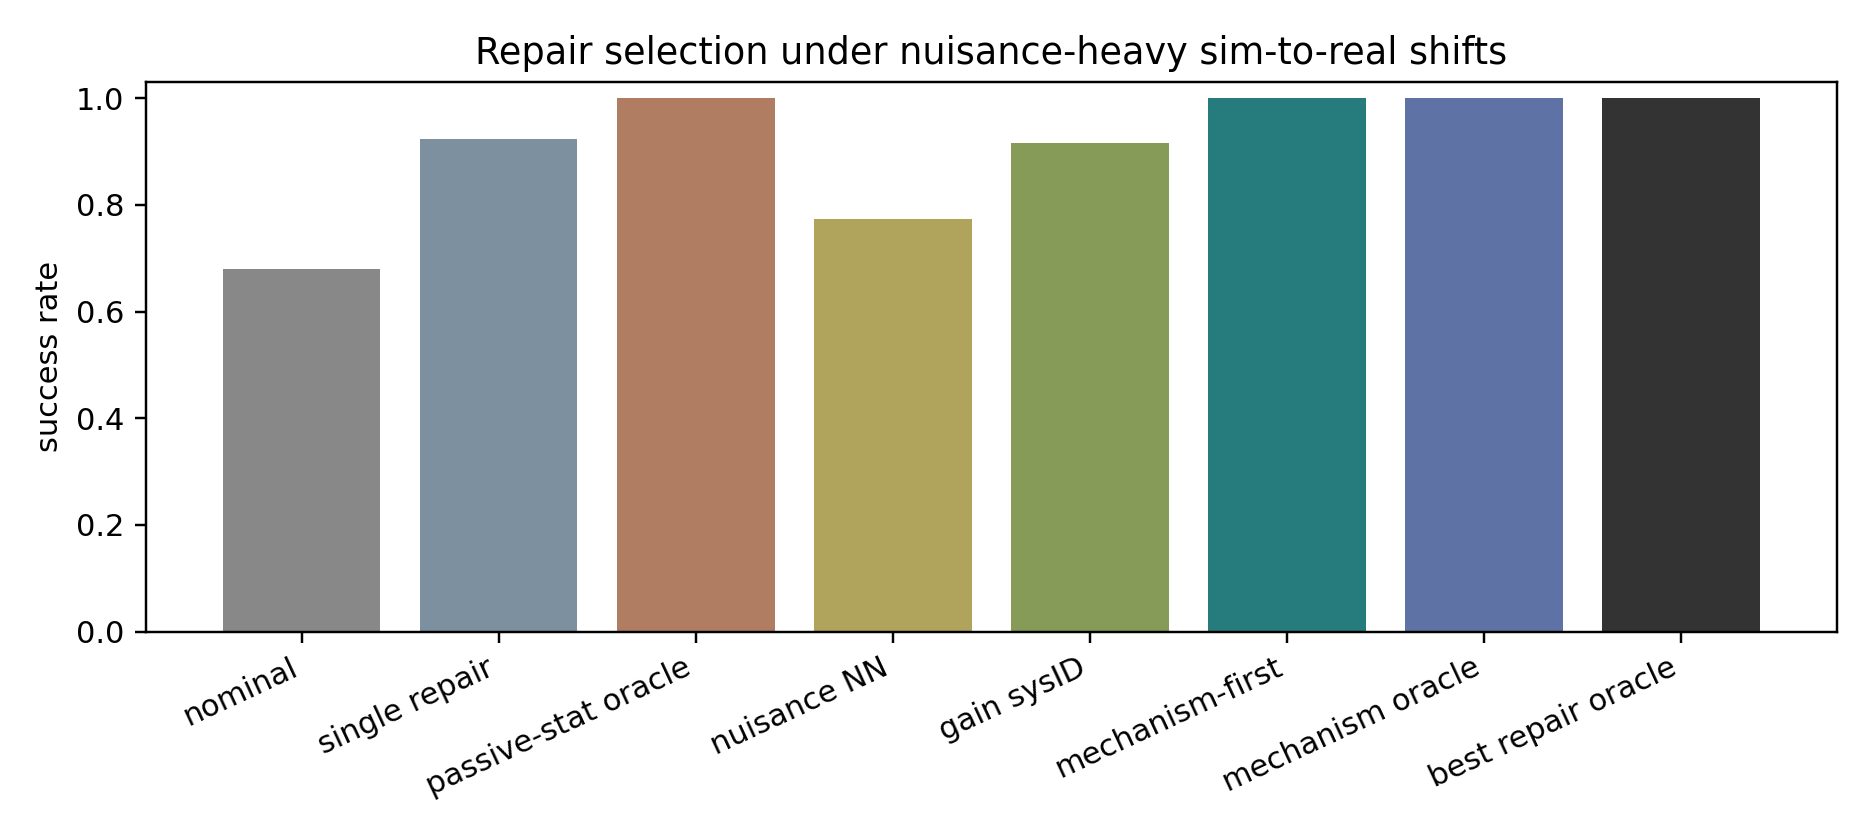
\includegraphics[width=0.94\linewidth]{../results/success_rates.png}
\caption{Thresholded success rates for all methods. The passive-statistic oracle reaches the loose success threshold, but Table~\ref{tab:results} shows worse final error than mechanism-first repair selection.}
\label{fig:success}
\end{figure}

\paragraph{Results.}
Mechanism-first probing matches the mechanism oracle on this run. It improves mean final error by about $4.5\times$ compared with the passive-statistic oracle and by more than $50\times$ compared with nuisance nearest neighbor. The probe classifier is perfect in the clean saved run, with all 1200 test domains assigned to the correct mechanism. Mechanism-level results show where generic coordinates break: gain-only system identification fails under slip, no adaptation fails under delay, and nuisance nearest neighbor is especially brittle under delay and slip.

\begin{table}[t]
\centering
\caption{Probe-noise stress over five repeats per noise level. The clean
hand-designed probe classifier is perfect, but mechanism-first repair degrades
as diagnostic residuals become noisy.}
\label{tab:probe-noise}
\begin{tabular}{lrrrrrr}
\toprule
Metric & 0.00 & 0.01 & 0.02 & 0.04 & 0.08 & 0.12 \\
\midrule
Mechanism accuracy & 1.000 & 1.000 & 0.982 & 0.830 & 0.608 & 0.503 \\
Success & 1.000 & 1.000 & 0.998 & 0.967 & 0.880 & 0.825 \\
Mean final error & 0.0017 & 0.0017 & 0.0038 & 0.0294 & 0.0786 & 0.1098 \\
\bottomrule
\end{tabular}

\end{table}

Table~\ref{tab:probe-noise} adds Gaussian noise to the diagnostic residual
features before mechanism classification. At $\sigma=0.02$, mechanism accuracy
is still 0.982 and mean final error is 0.0038. At $\sigma=0.04$, accuracy drops
to 0.830 and mean final error rises to 0.0294, worse than the clean passive
statistic oracle's 0.0076. At $\sigma=0.12$, mechanism accuracy is 0.503 and
mean final error is 0.1098. The claim is therefore conditional on reliable
diagnostic probes; mechanism-first coordinates do not solve probe design or
noisy mechanism identification.

\paragraph{Counterexample artifact.}
The repository includes a two-domain aliasing construction in \texttt{results/aliasing\_counterexample.csv}. Domain A has actuator gain loss and is repaired by gain compensation. Domain B has high-command contact slip and is repaired by slip-safe control. Both expose the same passive statistic $s=0.50$. Any adapter observing only $s$ must choose the same repair for both, so it fails on at least one.

\section{Limitations}

The strongest limitation is evidence scale. The simulator is intentionally small and diagnostic; it is not a hardware benchmark. The mechanism library is closed and hand-designed. The probes are also hand-designed, which means the paper does not solve probe synthesis. The v2 probe-noise stress makes this limitation concrete: once diagnostic residuals are noisy enough, the mechanism classifier misidentifies repair classes and the advantage over passive summaries can disappear. The passive-statistic baseline is representation-limited by construction; the formal proposition justifies studying that setting, but the experiment should not be read as a defeat of all passive or learned representations. Finally, real sim-to-real failures can be coupled, nonstationary, and out of library.

\section{Conclusion}

The paper changes the central adaptation variable from domain statistics to repair mechanisms. This change exposes a simple but important boundary: statistics that are predictive of domain identity or nominal rollout behavior can still be insufficient for repair selection. Mechanism-first probes offer a constructive alternative in a stylized contact-control setting. The next step is to test whether the same repair-equivalence view helps on hardware, especially in contact-rich manipulation where delay, slip, compliance, and sensing artifacts are common and costly to confuse.

\bibliography{references}
\bibliographystyle{iclr2026_conference}

\appendix
\section{Artifact Notes}

The repository includes the literature matrix, hostile prior-work set, simulator, cached results, and audit files. To rerun the experiment, execute \texttt{python experiments\textbackslash mechanism\_first\_sim.py} from the repository root. The expected aggregate results are written to \texttt{results\textbackslash summary.csv}. The final audit identifies unsupported claims and assigns the paper-readiness judgment.

\end{document}
